\documentclass[../main/thesis.tex]{subfiles}
\begin{document}
\newchapter
%% Electronics

\chapter{Readout Electronics for the 3DMiMic Detectors}
\label{e}
 

\section{Detector Readout}
\label{t-read}
In different situations, the desired output from the detector readout will be different. In some cases, it is enough to simply count the radiation quanta, and in other cases one might want to read out a energy spectrum. In both cases the readout chain starts with a pre-amplifier that produces a voltage that is proportional to the radiation charge. The output from the pre-amplifier is sent to a shaping amplifier which converts the signal to a shape that is more suitable for the next component in the readout chain. This is to select the interesting pulses and convert the analog signal to a digital signal in one way or another. \citep[chap. 16]{Knoll}

\subsection{Pre-Amplifier}
\label{t-amp}
For most radiation detectors, the liberated charge is too small to be processed, which is why pre-amplifiers are needed in most detector readout chains. The pre-amplifier is located close to the detector to reduce noise. A pre-amplifier can be voltage-sensitive or charge-sensitive. A voltage-sensitive pre-amplifier has an output signal proportional to the input voltage, which will be proportional to the input charge if the detector capacitance is constant. This is not the case for semiconductor detectors where the capacitance may change with the operating parameters. A \gls{CSA} has an output signal that is independent of the input capacitance as long as the amplifier gain is high enough compared to a relationship between capacitances in the system. \citep[chap. 16]{Knoll}
%fig 16.13?

One, often important, parameter to consider in a pre-amplifier is the dynamic range, which is the range of input signal amplitudes that can be reliably measured without changing the system. The lowest measurable input signal is limited by the noise in the system, mainly in the detector, detector cables, and pre-amplifier. A signal is not reliable if it is difficult to discern from the noise. The highest measurable input signal can be limited by the pre-amplifier or later stages, like the \gls{ADC}. If the pre-amplifier has a high gain, then a large input signal will require a higher output signal than the pre-amplifier can deliver. If the gain is low, then another stage in the system will likely be the bottleneck before the pre-amplifier reaches its highest output level. \citep{dynamic-range}

It is typically convenient to use the pre-amplifier to supply bias voltage to the detector. When this is done a single cable is used both to provide voltage to the detector and to transfer the signal pulses to the readout system. \citep[chap. 16]{Knoll}
%fig 16.16a?


\subsubsection{Charge-sensitive amplifier operation}
\label{t-csa}
\begin{figure}%[h]
	\centering
	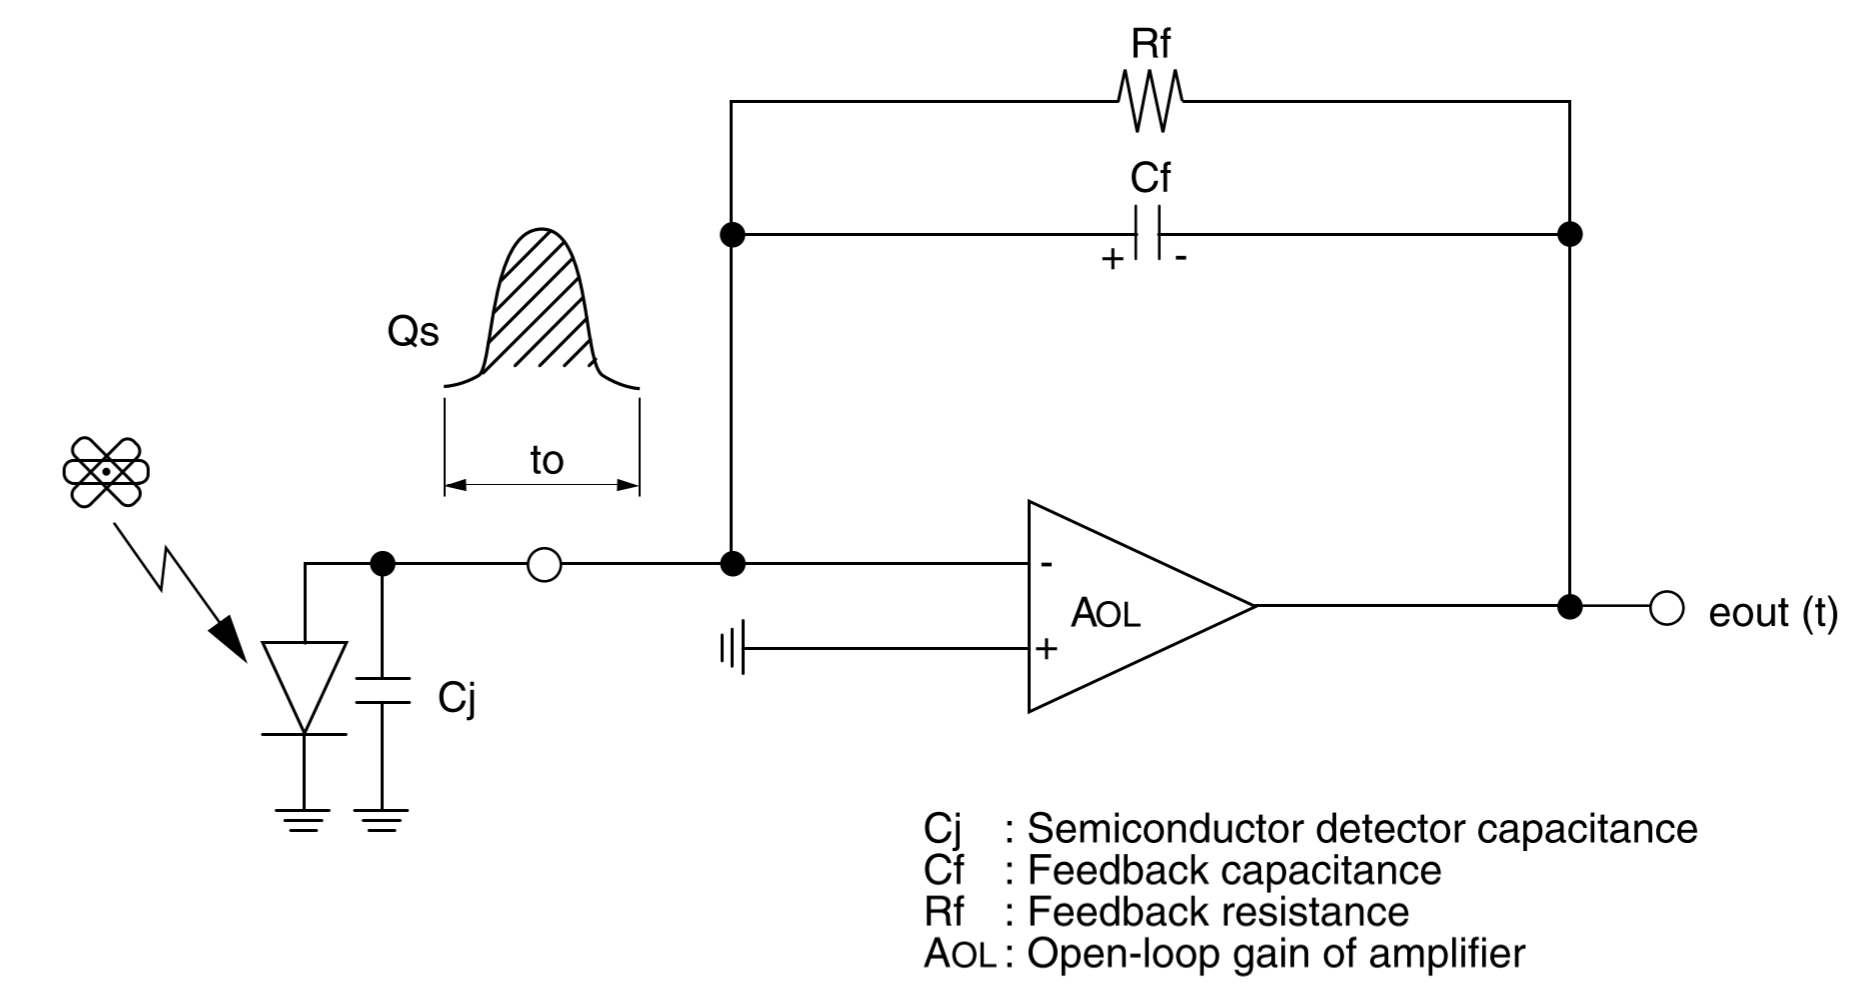
\includegraphics[width=\textwidth]{csa.png}
	\caption{Schematic of a basic \gls{CSA}. \citep{Hamamatsu}}
	\label{fig-csa}
\end{figure}

Figure \ref{fig-csa} shows a general \gls{CSA}. When a radiation quanta strikes the detector, a pulse of charge $Q_s$ and width $t_o$ is generated. This creates a rising potential on the negative input of the amplifier, which triggers a falling potential on the output of the amplifier. Because of the negative feedback, this will quickly draw the negative input close to zero, making it a point of virtual ground. The feedback currents charge the feedback capacitor, and then the capacitor is slowly discharged when there is no signal on the input. This creates a voltage pulse on the output that slowly falls from a peak value that is proportional to the input charge (figure \ref{fig-preampshaper}). \citep{Hamamatsu}

%http://www.allaboutcircuits.com/textbook/semiconductors/chpt-8/differentiator-integrator-circuits/
%Virtual ground: http://electronics.stackexchange.com/questions/124709/op-amp-reason-for-virtual-ground

%%XXX figure with pulse?
%%XXX basic noise stuff too? 

Since noise affects the resolution and dynamic range of a readout system, it is common to document the noise of an amplifier as \textit{input referred noise}. This is the equivalent noise on the input of the amplifier that would create the noise that is seen on the output. This is done to more easily compare the noise to the expected signal strength at the input. For a charge-sensitive amplifer, it is then natural to refer to the noise as the \acrfull{ENC} on the input.  

\subsection{Shaper}
\label{t-shaper}
The shaper, or shaping amplifier, converts the shape of the signal from the pre-amplifier to a form that is suitable for measurement.  It is important that the output from the shaper quickly returns to the baseline to prevent pulse overlapping that will cause measurement errors. The first stage of a simple shaper, figure \ref{fig-preampshaper}, is a differentiator (high pass filter) which passes the steep rise of the input pulse, but quickly returns to the baseline, and also reduces the noise. The differentiator decides the fall time of the pulse. The signal is then amplified to a level that is suitable for the \gls{ADC}, before it is passed through the integrator (low pass filter) that filters away noise and increases the rise time of the pulse. This simple shaper is often called a CR-RC shaper, from the electronic components it is made from. \citep[chap. 16]{Knoll}

\begin{figure}%[h]
	\centering
	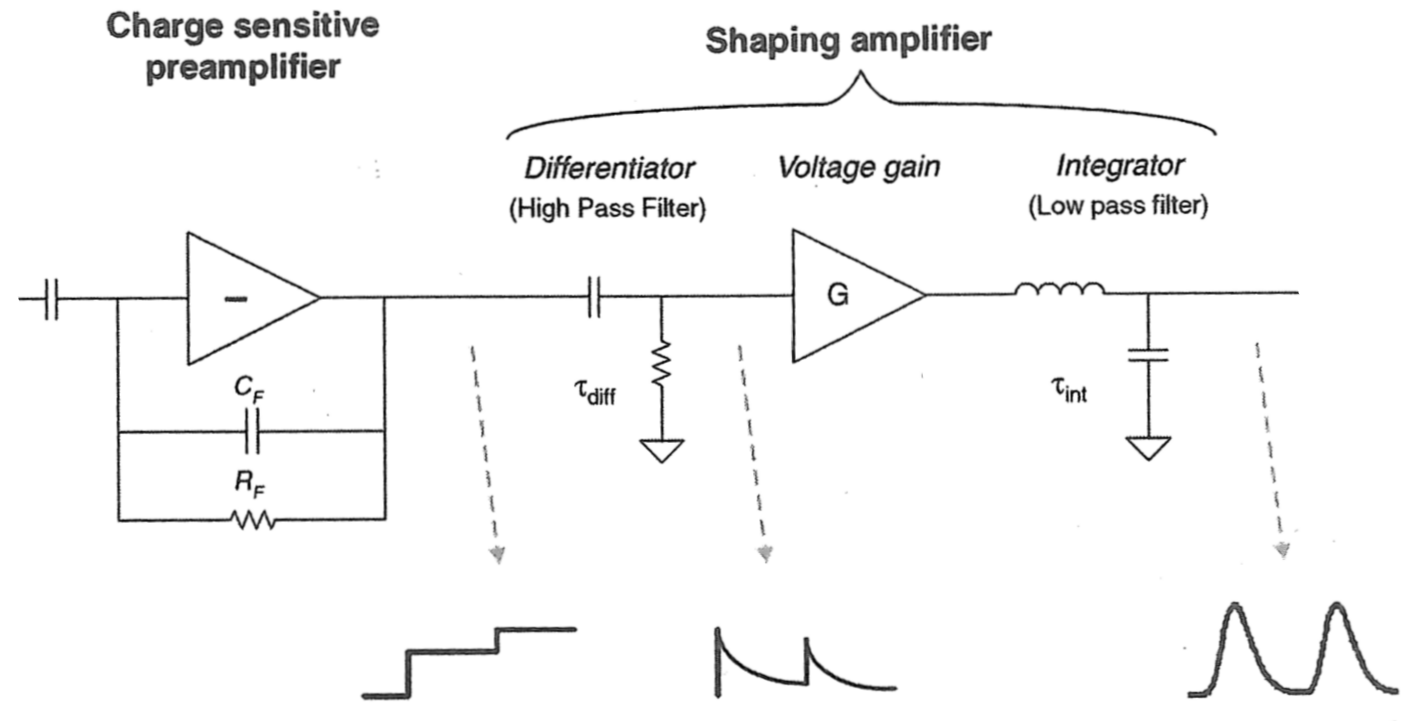
\includegraphics[width=0.8\textwidth]{preampshaper2.png}
	\caption{Schematic of simple charge sensitive pre-amplifier and shaper. Includes sketches of how the signal could look at different stages. \citep[chap. 16]{Knoll} }
	\label{fig-preampshaper}
\end{figure} %fig 16.2

A much used parameter to describe a shaper is the shaping time, which is related to the duration of the shaped pulse. There is no standard for defining what shaping time is, but common practice is to use the (shaping) time constant ($\tau=RC$) of the filters, even though this does not clearly define all the time-related parameters. \citep[chap. 17]{Knoll} Since the shaping time constant is defined by the electronic components in the shaper, it is not possible to use this definition when measuring the shaping time of a shaper with unknown design. Therefore, in this thesis, the shaping time definition from \citep{shapingtimedef} is used. This is the time difference between the peak and 61 \% of the peak value on the falling edge (figure \ref{fig-shapingtime-def}).  

\begin{figure}%[h]
	\centering
	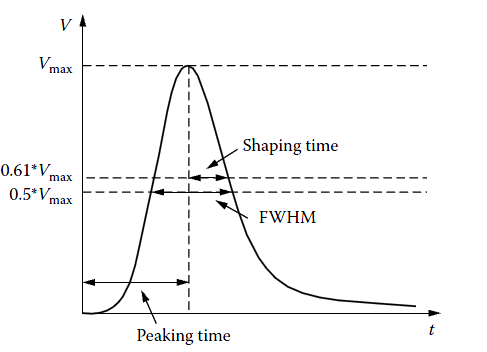
\includegraphics[width=0.6\textwidth]{shapingtime.png}
	\caption{Definition of shaping time and peaking time. \citep{shapingtimedef} }
	\label{fig-shapingtime-def}
\end{figure}

There are many factors that come into play when deciding the shaping time. A short shaping time is needed to avoid subsequent pulses to overlap (pile-up), but a too short shaping time can lead to an error called ballistic deficit. This is when a too short shaping time compared to the rise time of the input pulse leads to a decrease in amplitude. When the shaping time is too short, not all of the charge will have had time to be collected, and the output pulse does not reach the full amplitude. The signal-to-noise ratio is also affected by both the shape and the shaping time. At short shaping times, the series noise component of the pre-amplifier dominates the total noise. The series noise is typically dominated by thermal noise in the first amplifying stage of the pre-amplifier. At long shaping times the parallel noise dominates. This could for example be detector leakage current, transistor leakage current, and thermal noise in the pre-amplifier feedback resistor. To total noise has a minimum where the series and parallel noise is equal, see figure \ref{fig-noise-min}. This is typically at 0.5 to 1 $\mu$s for semiconductor particle detectors. \citep{ORTEC}
XXX fig ballistic deficit
\begin{figure}%[h]
	\centering
	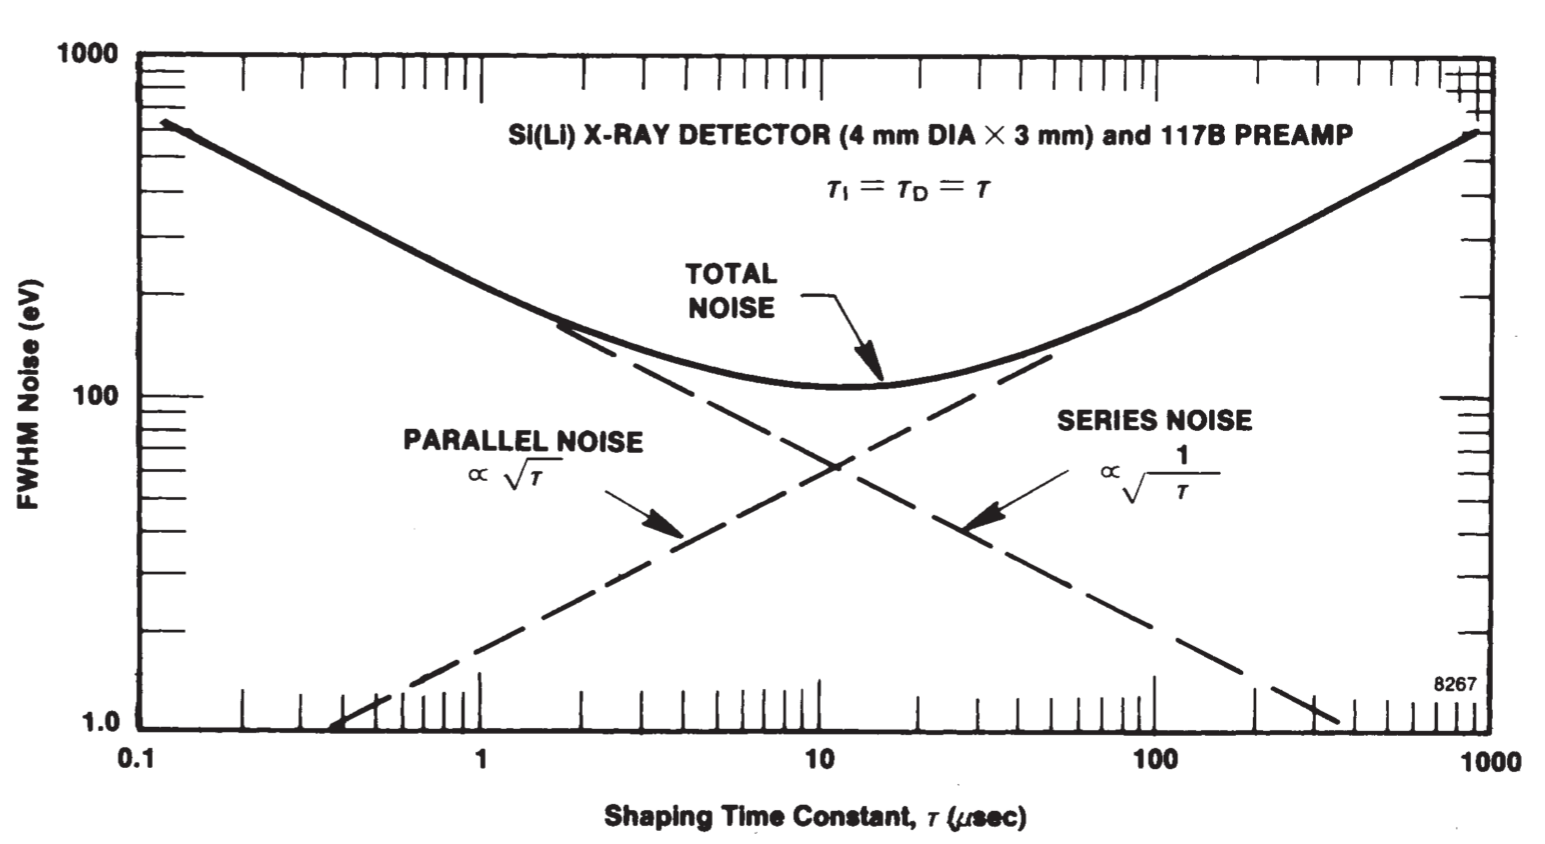
\includegraphics[width=0.6\textwidth]{noisemin.png}
	\caption{Noise versus shaping time. \citep{ORTEC} }
	\label{fig-noise-min}
\end{figure}

There are many other shaper configurations that can be used to create different shapes. One very popular choice is the CR-(RC)$^4$ shaper, which uses fourth order low pass filter to make the pulse shape an almost perfect Gaussian. This type of shaper is therefore often called a semi-Gaussian shaper. A CR-(RC)$^4$ shaper has about 18 \% higher signal-to-noise ratio, and about 11 \% lower deadtime than a CR-RC shaper. The fourth order filter can be implemented either by cascading four passive RC stages, or two active second order low pass filters. \citep{ORTEC} \citep[chap. 17]{Knoll}

Most shapers include a pole-zero cancellation network (figure \ref{fig-shaper-pz}) to remove an undershoot that is often seen after the pulse. This makes it possible to have higher counting rates without problems with pile-up. Pole-zero cancellation is done with a potentiometer in parallel with the capacitor in the CR differentiator. The name comes from the poles and zeroes in the transfer function of the system. The network uses a zero to cancel out a pole in the complex plane. \citep{ORTEC}

\begin{figure}%[h]
	\centering
	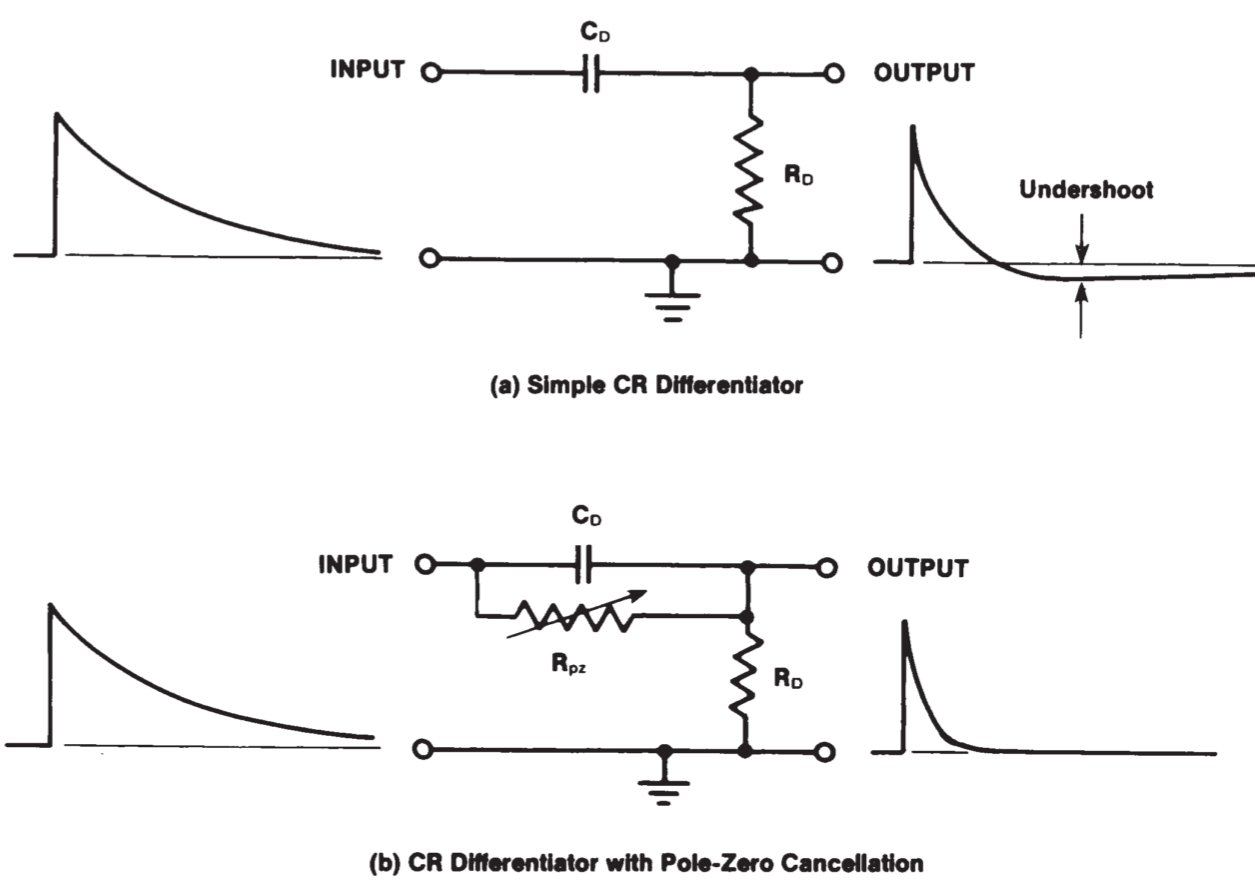
\includegraphics[width=0.7\textwidth]{pz.png}
	\caption{The benefit of Pole-Zero Cancellation. \citep{ORTEC} }
	\label{fig-shaper-pz}
\end{figure}

%%XXXX: More details. Noise. Ballistic deficit. semi-gauss shape. pz
%discriminator?
%% Figure with pulse from pre-amp and from shaper
%Shaping time definition

\subsection{Analog-to-Digital Conversion}
\label{t-adc}
The analog signal from the shaper needs to be converted to a digital signal for processing and storage. When it is desired to keep as much information as possible, an \gls{ADC} is used, but these use a lot of area and power. In situations where area, power, and cost is more important than accuracy of measurements (typically when there are a lot of channels), there are some simpler methods that can be used instead. The simplest is a counter, which merely counts the number of pulses with a height above a defined threshold. The information on the radiation quanta energy is lost, but the circuit is very simple. It is also possible to have multiple counters with different thresholds, which will keep some information about the distribution of radiation quanta energies. Another much used method is the \gls{ToT} technique. A \gls{ToT} circuit measures the time that the pulse is over a defined threshold, and then this measurement can be used to estimate the height of the pulse. The relationship between pulse height and \gls{ToT} is only linear within a certain range, and will usually limit the dynamic range of the readout system. \citep[chap. 6]{ToT}

%This link for ADC vs ToT: https://books.google.no/books?id=DFDRBQAAQBAJ&pg=PA173&lpg=PA173&dq=time+over+threshold+energy+measurement&source=bl&ots=J7wJ9nACVW&sig=ra60jHHnJxCc7g3g1TV2RLwHjqU&hl=en&sa=X&ved=0CBsQ6AEwADgKahUKEwi-zcfjuZTJAhUKnnIKHSQ4BAI#v=onepage&q=time%20over%20threshold%20energy%20measurement&f=false

An \gls{ADC} samples the analog signal amplitude at a certain interval (sampling rate) and converts each sampled value to a digital signal. The resolution, which is the number of bits in the digital signal, will limit the accuracy of the conversion. The quantisation error is introduced as each analog value needs to be converted to the closest digital value. The maximum percentage quantisation error can be seen in equation \ref{eq-eqmax}, where n is the number of digits in the binary code and $2^n$ is the number of digital values. \citep[chap. 10]{Bentley}

\begin{equation}%[h]
e_q^{MAX} = \pm \frac{100}{2(2^n - 1)}\%
\label{eq-eqmax}
\end{equation}

The dynamic range of an \gls{ADC} will mainly be limited by its resolution, noise, linearity, and jitter (small timing errors). This can be summarized with \gls{ENOB} to give a measure of the effective resolution, after noise and distortions. \gls{ENOB} is defined as the resolution of an ideal \gls{ADC} that would have the same effective resolution as the \gls{ADC} in question.
 %https://en.wikipedia.org/wiki/Analog-to-digital_converter
%Types of ADC?

\comm{
\subsection{Digital Signal Processing}
\label{t-dsp}
}

%\subsection{Medipix}
%\label{t-medipix}

\section{Choice of Readout Electronics for the 3DMiMic Detectors}

An overview of all readout electronics systems that was considered for use during this project can be found with relevant specifications in appendix \ref{a-asics}. The most promising systems are discussed and evaluated in this section. 

\subsection{Medipix and Timepix}
\label{e-medipix}
Medipix is a family of chips developed to exploit technology from the experiments at CERN in other fields of science, mainly medical imaging. The chips made by the Medipix collaboration are; Medipix1, Medipix2, Timepix, Medipix3, Timepix3, and Dosepix. The Medipix 1-3 chips are made for photon counting and are therefore not useful for dosimetry. The Timepix chips are made to do \gls{ToT} measurements, with Timepix and Timepix3 being based on Medipix2 and Medipix3 respectively. Dosepix is a currently in development chip made for photon dosimetry. They have extremely good noise properties, down to 60~e- of noise without a detector connected for Timepix3. Timepix3 and Dosepix were considered for the 3DMiMic project, but as \gls{ToT} devices their dynamic range is not very large. Also, since they are made for photon detectors they cannot read the largest charges (table \ref{tab-3d-response}) that can be expected from the 3DMiMic detectors. \citetext{\citeauthor{Medipix}}

\subsection{UiO Portable Front-End Readout System}
\label{e-uio}
During the school year 2014-2015 two master students at \gls{uio} made a portable front-end readout system for radiation detectors \citep{tali} \citep{oltedal}. This system consists of two custom made cards and a \gls{FPGA} evaluation board. The first card, the analog card, has three channels with pre-amplifiers while two of those channels also including shapers. The second card, the digital card, includes an \gls{ADC}, comparators, and current monitors. The components of the digital card is connected to the \gls{FPGA} on the SoCKit evaluation board by Arrow, which is connected to a computer through network. The system is made to detect fission fragments which produce very large signals, and therefore has a low gain. This makes the system too noisy for the low noise requirements of the 3DMiMic detector at the default gain, but this can be changed using external components.

\subsection{IDEAS IDE1180 Amadeus Preamp-Shaper}
\label{e-ide1180}
IDE1180, or Amadeus, by Oslo-based IDEAS is an \gls{asic} for the front-end readout of radiation detectors. It features 16 channels of \gls{CSA} and shapers with adjustable shaping time. The preliminary datasheet \citep{IDE1180} specifies a shaping time between 20~ns and 40~ns, negative and positive input charges up to 400~fC with lowest gain, and equivalent noise charge of 1106~e- plus 68~e- per pF load at default gain. 

This chip was considered by multiple projects at \gls{ift} and a evaluation board (7045) was given to \gls{ift} so that more extensive tests could be performed. Later, a second evaluation board (7048) was also received from IDEAS. The IDE1180 characterization is described in chapter \ref{ide}. 

\subsection{Ortec 142A Pre-Amplifier}
\label{e-ortec}
Ortec 142A is a single channel low-noise \gls{CSA} optimized for charged particle or heavy-ion detectors. It was considered for the 3DMiMic project since \gls{uib} already owns a few of these. It features a very high dynamic range, up to 55~Me-, and an equivalent noise charge between 444~e- and 944~e- for detector capacitances between 0~pF and 100~pF. The University does not have a fitting portable shaping amplifier that can be used with the 142A, and it was therefore not prioritized for this project. The 142A is also well characterized and documented by Ortec. \citep{Ortecdata}

%but the gain is too low for the 3DMiMic detector. <-wrong

\section{Portable PCIe ADC System}
\label{e-adc}
The current \gls{ADC} system used at \gls{uib} is a Caen V1729A digitizer sitting in a VME crate. This features four 14 bit channels with 2~GS/s sampling rate, and 0.3 mV accuracy (125 $\mu$V quantisation error and 175 $\mu$V noise), but is very large and heavy, making it cumbersome to bring for radiation tests. It was decided to purchase a new \gls{ADC} for the department that could be put inside a small computer using \gls{PCIe} to make a portable system. Three manufacturers that produced suitable \gls{ADC}s for a reasonable price were found; AlazarTech, Keysight Technologies, and SP Devices. The considered models are listed in table~\ref{tab-adc}. 

\begin{table}[h]
\begin{center}
	\caption{The analog-to-digital converters considered for purchase.}
	\label{tab-adc}
	\begin{tabular}{ccccc}%{| c | c | c | c | c |}
		\toprule %\hline
		\textbf{Manufacturer} & \textbf{Mode}l & \textbf{Channels} & \textbf{Resolution} & \textbf{Sampling} \\ 
		 & & & (bits) & (GS/s) \\ \midrule%\hline
		AlazarTech & ATS9360 & 2 & 12 & 1.8 \\ %\hline
		Keysight & U5303A & 2 (1) & 12 & 1.6 (3.2) \\ %\hline
		SP Devices & ADQ14AC-2X & 2 & 14 & 2 \\ %\hline
		SP Devices & ADQ14AC-4C & 4 & 14 & 1 \\ \bottomrule%\hline
	\end{tabular}
\end{center}
\end{table}

The Keysight model was interesting with a signal interleaving feature where both 1.6~GS/s channels could be combined into one 3.2~GS/s channel. In the end SP Devices was chosen, being the only discovered company that produces 14 bit \gls{PCIe} \gls{ADC}s in the GS/s range. ADQ14AC-4C was chosen since having two extra channels was considered more important than higher sampling rate for radiation tests, and the old Caen \gls{ADC} can be used for projects and tests that require higher sampling rate. 

\subsection{SP Devices ADQ14AC-4C ADC}
\label{e-adc-pc}

The SP Devices ADQ14AC-4C has a input range of 1.9 $V_{pp}$ and has a variable DC offset of $\pm1.05$ V. It has an \gls{ENOB} of 10.2, which gives an accuracy of 1.62 mV. This gives it worse accuracy and sampling rate then the Caen ADC. 

A computer is needed to host the SP Devices \gls{ADC}. The main requirement for the computer is that it is able to transfer data over \gls{PCIe} close to the maximum data transfer rate of 3.2 GB/s specified in the ADQ14 datasheet. This puts requirements on the CPU, RAM, and motherboard. The CPU and motherboard needs to have eight available \gls{PCIe} 2.0 lanes for the ADQ14. In addition, the CPU, chipset, and BIOS needs to support a \gls{PCIe} payload size of 256 bytes. %However, this parameter is not something CPU and motherboard manufacturers typically supply in datasheets. Also, the CPU and RAM needs to be able to handle a high load from the ADC, operating system, and software. Since most of these requirements is not something you can check in the datasheet, the safest way to assure maximum performance is to buy a high-end CPU and motherboard, and a good amount of RAM.
%cite datasheet?

%bygge selv vs. Dell/HP
%The main choice in computers stood between buying individual components, or purchasing a computer through a deal the IT department has with the computer manufacturers. The benefits of buying individual components would be higher certainty that the motherboard has good enough performence, and possibilities to buy a chassis of desired size. The benefits of buying a computer through the IT department is extended warranty and help setting up software. In the end, HP~ProDesk~600~G2 with a micro-tower chassis was chosen. This has an Intel i7-6700 CPU, 64~GB of DDR4 RAM, a 256~GB SSD, and a 3~TB HDD. 
A HP~ProDesk~600~G2 with a micro-tower chassis has been purchased to be used with the new ADC. This has an Intel i7-6700 CPU, 64~GB of DDR4 RAM, a 256~GB SSD, and a 3~TB HDD. 


\end{document}